%!TEX root = ../template.tex
%%%%%%%%%%%%%%%%%%%%%%%%%%%%%%%%%%%%%%%%%%%%%%%%%%%%%%%%%%%%%%%%%%%%
%% chapter5.tex
%% NOVA thesis document file
%%
%% Chapter with lots of dummy text
%%%%%%%%%%%%%%%%%%%%%%%%%%%%%%%%%%%%%%%%%%%%%%%%%%%%%%%%%%%%%%%%%%%%

\typeout{NT FILE chapter5.tex}

\chapter{Case Studies}\label{cha:case-study}

In this chapter I present some case studies where my library was used and discuss some of its strengths and weaknesses.
This chapter's example's full code is available at \url{https://github.com/rustype/typestate-examples}.

\section{Ring}\label{sec:case-study:ring}

The ring example is taken out of the Rumpsteak \autocite{Cutner2021} repository.
The general example is composed of $N$ participants, in a \emph{ring},
where the first participant sends the value to the participant on the right,
the other participant receives the value from the left and each participant repeats the same process;
visualized in \autoref{fig:ring}.

\begin{figure}
    % STOLEN: https://texample.net/tikz/examples/cycle/
    % STOLEN: https://tex.stackexchange.com/questions/184852/use-array-in-loop-in-tikz
    % STOLEN: https://tex.stackexchange.com/questions/38763/how-to-place-a-node-in-the-middle-of-an-arc
    \centering
    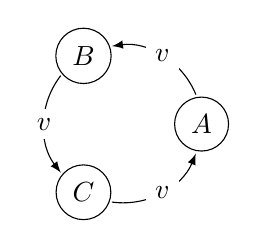
\begin{tikzpicture}
        \def \n {3}
        \def \radius {1cm}
        \def \margin {22} % margin in angles, depends on the radius

        \foreach[count=\s] \v in {A,B,C}
        {
        \node[draw, circle] at ({360/\n * (\s - 1)}:\radius) {$\v$};
        \draw[->, >=latex] ({360/\n * (\s - 1)+\margin}:\radius)
        arc ({360/\n * (\s - 1)+\margin}:{360/\n * (\s)-\margin}:\radius) node[midway, fill=white]{$v$} ;
        }
    \end{tikzpicture}
    \caption{The ring example visualization.}
    \label{fig:ring}
\end{figure}

Before comparing both APIs, it is important to notice that Rumpsteak is aimed at \gls{MPST}
for Rust's \texttt{async}/\texttt{await} syntax,
enabling the description and enforcement of communication patterns using the type system.
\textcolor{attrgreen}{\annotation{typestate}} was designed with typestates and API constraints in mind,
while it is unable to describe and enforce communication patterns,
it is able to enforce function call ordering at compile-time, avoiding API misuses.

Taking it a step further, consider \autoref{fig:ring},
Rumpsteak is enforces constraints on the edges of that graph \ie{\quotes{external} protocol},
such as where they come from and where they go to,
while \textcolor{attrgreen}{\annotation{typestate}} enforces constraints on the nodes \ie{\quotes{internal} protocol},
such as the possible steps the node will follow.

\subsection{Comparison}

\paragraph{Rumpsteak} first declares a series of types, the global type --- \textcolor{structblue}{\ttt{Roles}};
each participant endpoint --- \ttt{struct}s \textcolor{structblue}{\ttt{A}}, \textcolor{structblue}{\ttt{B}} and \textcolor{structblue}{\ttt{C}};
the message being passed around --- \textcolor{structblue}{\ttt{Value}};
finally, each session type --- \ttt{struct}s \textcolor{structblue}{\ttt{RingA}}, \textcolor{structblue}{\ttt{RingB}} and \textcolor{structblue}{\ttt{RingC}}.
The functionality of each participant is then declared as an \ttt{async} function,
notice that \ttt{ring\_b} (lines 32-39 from \autoref{lst:rumpsteak-ring})
and \ttt{ring\_c} (lines 41-48 from \autoref{lst:rumpsteak-ring}) are identical, except for the types used.

Given the session type nature of Rumpsteak, the library is able to enforce communication patterns at the type level,
In lines 19-21 of \autoref{lst:rumpsteak-ring} we can see through \ttt{RingA}'s type that
\ttt{A} will forcibly send the value to \ttt{B} and will then receive the value from \ttt{C};
this is not enforceable using \textcolor{attrgreen}{\annotation{typestate}}.

The launch routine \autoref{lst:rumpsteak-ring-main} is standard,
using the executor from the \ttt{future} crate along with the \ttt{try\_join} macro as a convenience to launch each one.
Rumpsteak ends up being fairly verbose \wrt~the used types,
although the final usage \ie{the \ttt{main} and \ttt{ring\_} functions} is straightforward.

\begin{listing}
    \centering
    \begin{minted}{Rust}
#[derive(Roles)]
struct Roles(A, B, C);

#[derive(Role)]
#[message(Value)]
struct A(#[route(B)] Sender, #[route(C)] Receiver);

#[derive(Role)]
#[message(Value)]
struct B(#[route(A)] Receiver, #[route(C)] Sender);

#[derive(Role)]
#[message(Value)]
struct C(#[route(A)] Sender, #[route(B)] Receiver);

#[derive(Message)]
struct Value(i32);

#[session] type RingA = Send<B, Value, Receive<C, Value, End>>;
#[session] type RingB = Receive<A, Value, Send<C, Value, End>>;
#[session] type RingC = Receive<B, Value, Send<A, Value, End>>;

async fn ring_a(role: &mut A, input: i32) -> Result<i32> {
    let x = input;
    try_session(role, |s: RingA<'_, _>| async {
        let s = s.send(Value(x)).await?;
        let (Value(y), s) = s.receive().await?;
        Ok((x + y, s))
    }).await
}

async fn ring_b(role: &mut B, input: i32) -> Result<i32> {
    let x = input;
    try_session(role, |s: RingB<'_, _>| async {
        let (Value(y), s) = s.receive().await?;
        let s = s.send(Value(x)).await?;
        Ok((x + y, s))
    }).await
}

async fn ring_c(role: &mut C, input: i32) -> Result<i32> {
    let x = input;
    try_session(role, |s: RingC<'_, _>| async {
        let (Value(y), s) = s.receive().await?;
        let s = s.send(Value(x)).await?;
        Ok((x + y, s))
    }).await
}
    \end{minted}
    \caption{Rumpsteak's Ring implementation.}
    \label{lst:rumpsteak-ring}
\end{listing}

\begin{listing}
    \begin{minted}{Rust}
fn main() {
    let Roles(mut a, mut b, mut c) = Roles::default();

    let input = (1, 2, 3);
    println!("input = {:?}", input);

    let output = executor::block_on(async {
        try_join!(
            ring_a(&mut a, input.0),
            ring_b(&mut b, input.1),
            ring_c(&mut c, input.2),
        )
        .unwrap()
    });
    println!("output = {:?}", output);
}
    \end{minted}
    \caption{Rumpsteak's Ring \ttt{main} function.}
    \label{lst:rumpsteak-ring-main}
\end{listing}

\paragraph{\annotation{typestate}} type usage requires less background knowledge than Rumpsteak,
a user that understands the \gls{DSL} should be able to understand what goes on \quotes{behind the scenes}.

In my example (\autoref{lst:typestate-ring-starter}, \autoref{lst:typestate-ring-follower},  \autoref{lst:typestate-ring-main})
the protocol is enforced by declaring the state machine of each participant;
in this case, while the ring can scale up to $N$ participants, only two protocols are required ---
one for the participant starting the value propagation,
and one for the all other participants, which need to receive the value first.
The participants typestates are visualized in \autoref{fig:ring-typestate}.

Both \textcolor{structblue}{\ttt{RingA}} and \textcolor{structblue}{\ttt{RingB}} receive two channels
(respectively, lines 12 \& 23-25 in \autoref{lst:typestate-ring-starter}, and lines 18 \& 38-40 in \autoref{lst:typestate-ring-follower}),
one from which they will receive the value, and one to which they will send the value,
these channels, respectively, connect to the previous and next participants in the ring;
the channels are received upon instantiation of the respective \textcolor{structblue}{\ttt{Ring}} object.

\textcolor{structblue}{\ttt{Ring}A} (\autoref{lst:typestate-ring-starter}) starts the process,
thus, it is the only participant starting in a \emph{sending} state
(lines 10-16, emphasizing line 12, which declares the initial state);
in this state the \gls{API} allows the client to inspect the value with \ttt{get\_value} (lines 13 \& 27);
transition to the next state with \ttt{send} (lines 14 \& 29-36);
or end the protocol with \ttt{end} (lines 15 \& 38).

Inversely to \textcolor{structblue}{\ttt{RingA}}, \textcolor{structblue}{\ttt{RingB}} will first receive the value,
as it would be the participant next to the first sender and thus all other participants;
conversely, the protocol (\autoref{lst:typestate-ring-follower}) will start in a \emph{receiving} state
(lines 16-21, emphasizing line 18, which declares the initial state).
The main difference from \textcolor{structblue}{\ttt{RingA}} to \textcolor{structblue}{\ttt{RingB}} is the initial state, the inner logic is the same
and besides \ttt{new} (lines 18 \& 38-40) and \ttt{end} (lines 20 \& 51), other functions belong to the same states.

While \textcolor{attrgreen}{\annotation{typestate}} is unable to enforce communication patterns,
it is able to reuse the participants more effectively \ie{who sends to whom};
given that \textcolor{structblue}{\ttt{B}} and \textcolor{structblue}{\ttt{C}} perform the same operations, we can simply reuse \textcolor{structblue}{\ttt{RingB}} (\autoref{lst:typestate-ring-follower})
for both \textcolor{structblue}{\ttt{B}} and \textcolor{structblue}{\ttt{C}} (lines 7-8 of \autoref{lst:typestate-ring-main}).

\subsection{Summary}

As previously stated, Rumpsteak allows the developer to enforce communication patterns at compile-time,
while \textcolor{attrgreen}{\annotation{typestate}} does not, however, the latter is able to enforce behavior patterns at the participant level;
\textcolor{attrgreen}{\annotation{typestate}} is thus more flexible, being usable in synchronous or parallel programming,
while Rumpsteak was designed with \ttt{async}/\ttt{await} in mind.

It is important to note that in both cases (\autoref{lst:rumpsteak-ring} and \autoref{lst:typestate-ring-main})
there is opportunity to improve modularity,
one can use macros to abstract over the mostly repeated bits of code.
For \textcolor{attrgreen}{\annotation{typestate}}, for example, one can define a macro like \autoref{lst:typestate-ring-macro} and
shorten the lines 17-28 in \autoref{lst:typestate-ring-main} into lines 17 \& 18 in \autoref{lst:typestate-ring-main-macro}.


\begin{figure}
    \centering
    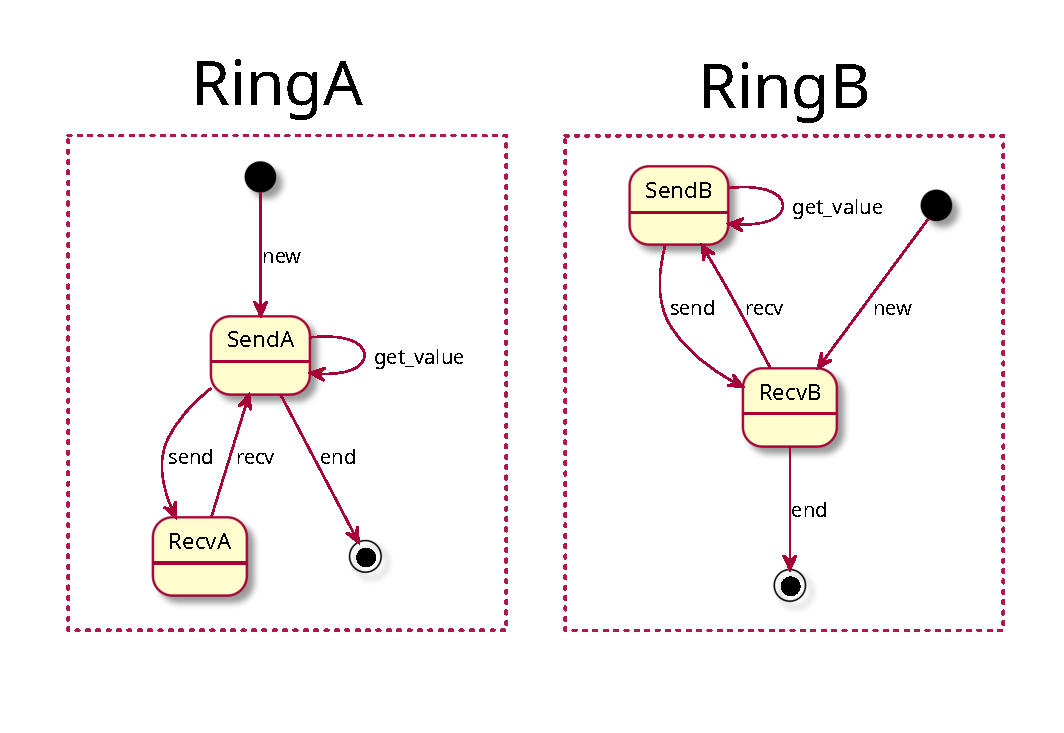
\includegraphics[width=\linewidth]{Chapters/Figures/C5/rings.pdf}
    \caption{The ring participants' typestates.}
    \label{fig:ring-typestate}
\end{figure}

\begin{listing}
    \begin{minted}{Rust}
#[typestate]
mod ring_a {
    use std::sync::mpsc::{Receiver, Sender};

    #[automaton] pub struct RingA {
        pub(crate) send: Sender<i32>,
        pub(crate) receiver: Receiver<i32>,
    }

    #[state] pub struct SendA(pub i32);
    pub trait SendA {
        fn new(value: i32, send: Sender<i32>, receiver: Receiver<i32>) -> SendA;
        fn get_value(&self) -> i32;
        fn send(self) -> RecvA;
        fn end(self);
    }

    #[state] pub struct RecvA;
    pub trait RecvA { fn recv(self) -> SendA; }
}

impl SendAState for RingA<SendA> {
    fn new(value: i32, send: Sender<i32>, receiver: Receiver<i32>) -> Self {
        Self { send, receiver, state: SendA(value) }
    }

    fn get_value(&self) -> i32 { self.state.0 }

    fn send(self) -> RingA<RecvA> {
        self.send.send(self.state.0).unwrap();
        RingA::<RecvA> {
            send: self.send,
            receiver: self.receiver,
            state: RecvA,
        }
    }

    fn end(self) {}
}

impl RecvAState for RingA<RecvA> {
    fn recv(self) -> RingA<SendA> {
        let value = self.receiver.recv().unwrap();
        RingA::<SendA> {
            send: self.send,
            receiver: self.receiver,
            state: SendA(value),
        }
    }
}
    \end{minted}
    \caption{\textcolor{attrgreen}{\annotation{typestate}}'s implementation of participant A.}
    \label{lst:typestate-ring-starter}
\end{listing}

\begin{listing}
    \begin{minted}{Rust}
#[typestate]
mod ring_b {
    use std::sync::mpsc::{Receiver, Sender};
    #[automaton]
    pub struct RingB {
        pub(crate) send: Sender<i32>,
        pub(crate) receiver: Receiver<i32>,
    }

    #[state] pub struct SendB(pub i32);
    pub trait SendB {
        fn get_value(&self) -> i32;
        fn send(self) -> RecvB;
    }

    #[state] pub struct RecvB;
    pub trait RecvB {
        fn new(send: Sender<i32>, receiver: Receiver<i32>) -> RecvB;
        fn recv(self) -> SendB;
        fn end(self);
    }
}

impl SendBState for RingB<SendB> {
    fn get_value(&self) -> i32 { self.state.0 }

    fn send(self) -> RingB<RecvB> {
        self.send.send(self.state.0).unwrap();
        RingB::<RecvB> {
            send: self.send,
            receiver: self.receiver,
            state: RecvB,
        }
    }
}

impl RecvBState for RingB<RecvB> {
    fn new(send: Sender<i32>, receiver: Receiver<i32>) -> Self {
        Self { send, receiver, state: RecvB }
    }

    fn recv(self) -> RingB<SendB> {
        let value = self.receiver.recv().unwrap();
        RingB::<SendB> {
            send: self.send,
            receiver: self.receiver,
            state: SendB(value),
        }
    }

    fn end(self) {}
}
    \end{minted}
    \caption{\textcolor{attrgreen}{\annotation{typestate}}'s implementation of participant B.}
    \label{lst:typestate-ring-follower}
\end{listing}

\begin{listing}
    \begin{minted}{rust}
fn main() {
    let (a_sender, b_receiver) = channel::<i32>();
    let (b_sender, c_receiver) = channel::<i32>();
    let (c_sender, a_receiver) = channel::<i32>();

    let a = RingA::<SendA>::new(0, a_sender, a_receiver);
    let b = RingB::<RecvB>::new(b_sender, b_receiver);
    let c = RingB::<RecvB>::new(c_sender, c_receiver);

    vec![
        thread::spawn(move || {
            println!("a: {}", a.get_value());
            let a = a.send();
            let a = a.recv();
            a.end();
        }),
        thread::spawn(move || {
            let b = b.recv();
            println!("b: {}", b.get_value());
            let b = b.send();
            b.end();
        }),
        thread::spawn(move || {
            let c = c.recv();
            println!("c: {}", c.get_value());
            let c = c.send();
            c.end();
        }),
    ]
    .into_iter()
    .map(|handle| handle.join())
    .collect::<Result<_, _>>()
    .unwrap()
}
    \end{minted}
    \caption{The \ttt{main} implementing for \textcolor{attrgreen}{\annotation{typestate}}'s ring.}
    \label{lst:typestate-ring-main}
\end{listing}

\begin{listing}
    \begin{minted}{rust}
macro_rules! spawn_ring_b {
    ($ring:ident) => {
        thread::spawn(move || {
            let $ring = $ring.recv();
            println!("{}: {}", stringify!($ring), $ring.get_value());
            let $ring = $ring.send();
            $ring.end();
        })
    };
}
    \end{minted}
    \caption{\ttt{macro\_rules!} to abstract over the thread launching routing for \textcolor{structblue}{\ttt{RingB}}.}
    \label{lst:typestate-ring-macro}
\end{listing}

\begin{listing}
    \begin{minted}{rust}
fn main() {
    let (a_sender, b_receiver) = channel::<i32>();
    let (b_sender, c_receiver) = channel::<i32>();
    let (c_sender, a_receiver) = channel::<i32>();

    let a = RingA::<SendA>::new(0, a_sender, a_receiver);
    let b = RingB::<RecvB>::new(b_sender, b_receiver);
    let c = RingB::<RecvB>::new(c_sender, c_receiver);

    vec![
        thread::spawn(move || {
            println!("a: {}", a.get_value());
            let a = a.send();
            let a = a.recv();
            a.end();
        }),
        spawn_ring_b!(b),
        spawn_ring_b!(c),
    ]
    .into_iter()
    .map(|handle| handle.join())
    .collect::<Result<_, _>>()
    .unwrap()
}
    \end{minted}
    \caption{The \ttt{main} implementing for \textcolor{attrgreen}{\annotation{typestate}}'s ring using \autoref{lst:typestate-ring-macro}.}
    \label{lst:typestate-ring-main-macro}
\end{listing}

\section{PIN}\label{sec:case-study:pin}

The PIN example has three principals, a card (\autoref{lst:typestate-card}),
read by the card reader (\autoref{lst:typestate-reader}), which is used by the final client.

To use the card, the reader ensures that the card is present by calling \ttt{check\_for\_card}
(line 10 of \autoref{lst:typestate-reader});
in the case the card is not present the reader transitions to the \textcolor{structblue}{\ttt{Error}} state,
otherwise, the reader transitions to the \textcolor{structblue}{\ttt{CardPresent}} state (line 13 of \autoref{lst:typestate-reader}).
The \textcolor{structblue}{\ttt{CardPresent}} state not only requires a reference to the card,
but also that the card itself is in the \textcolor{structblue}{\ttt{Start}} state (line 14 of \autoref{lst:typestate-reader}
and lines 8-13 of \autoref{lst:typestate-card}).
From the \textcolor{structblue}{\ttt{CardPresent}} state, the reader can issue an authentication operation,
which is done by the card by checking the PIN against the on stored inside the card;
if the authentication succeeds, the card reference is now required to reflect the reader's state,
enforcing that the card is also in the \textcolor{structblue}{\ttt{Authenticated}} state
(line 21 of \autoref{lst:typestate-reader} and lines 15-19 of \autoref{lst:typestate-card});
this relationship is visualized in \autoref{fig:reader-card-typestates}.

Any client of the reader API is thus required to check all steps before proceeding with the card.
The state embedding also guarantees that the \textcolor{structblue}{\ttt{Reader}} is a well-behaved client of the \textcolor{structblue}{\ttt{Card}},
similar to Fugue \autocite{DeLine2004}.

\begin{figure}
    \centering
    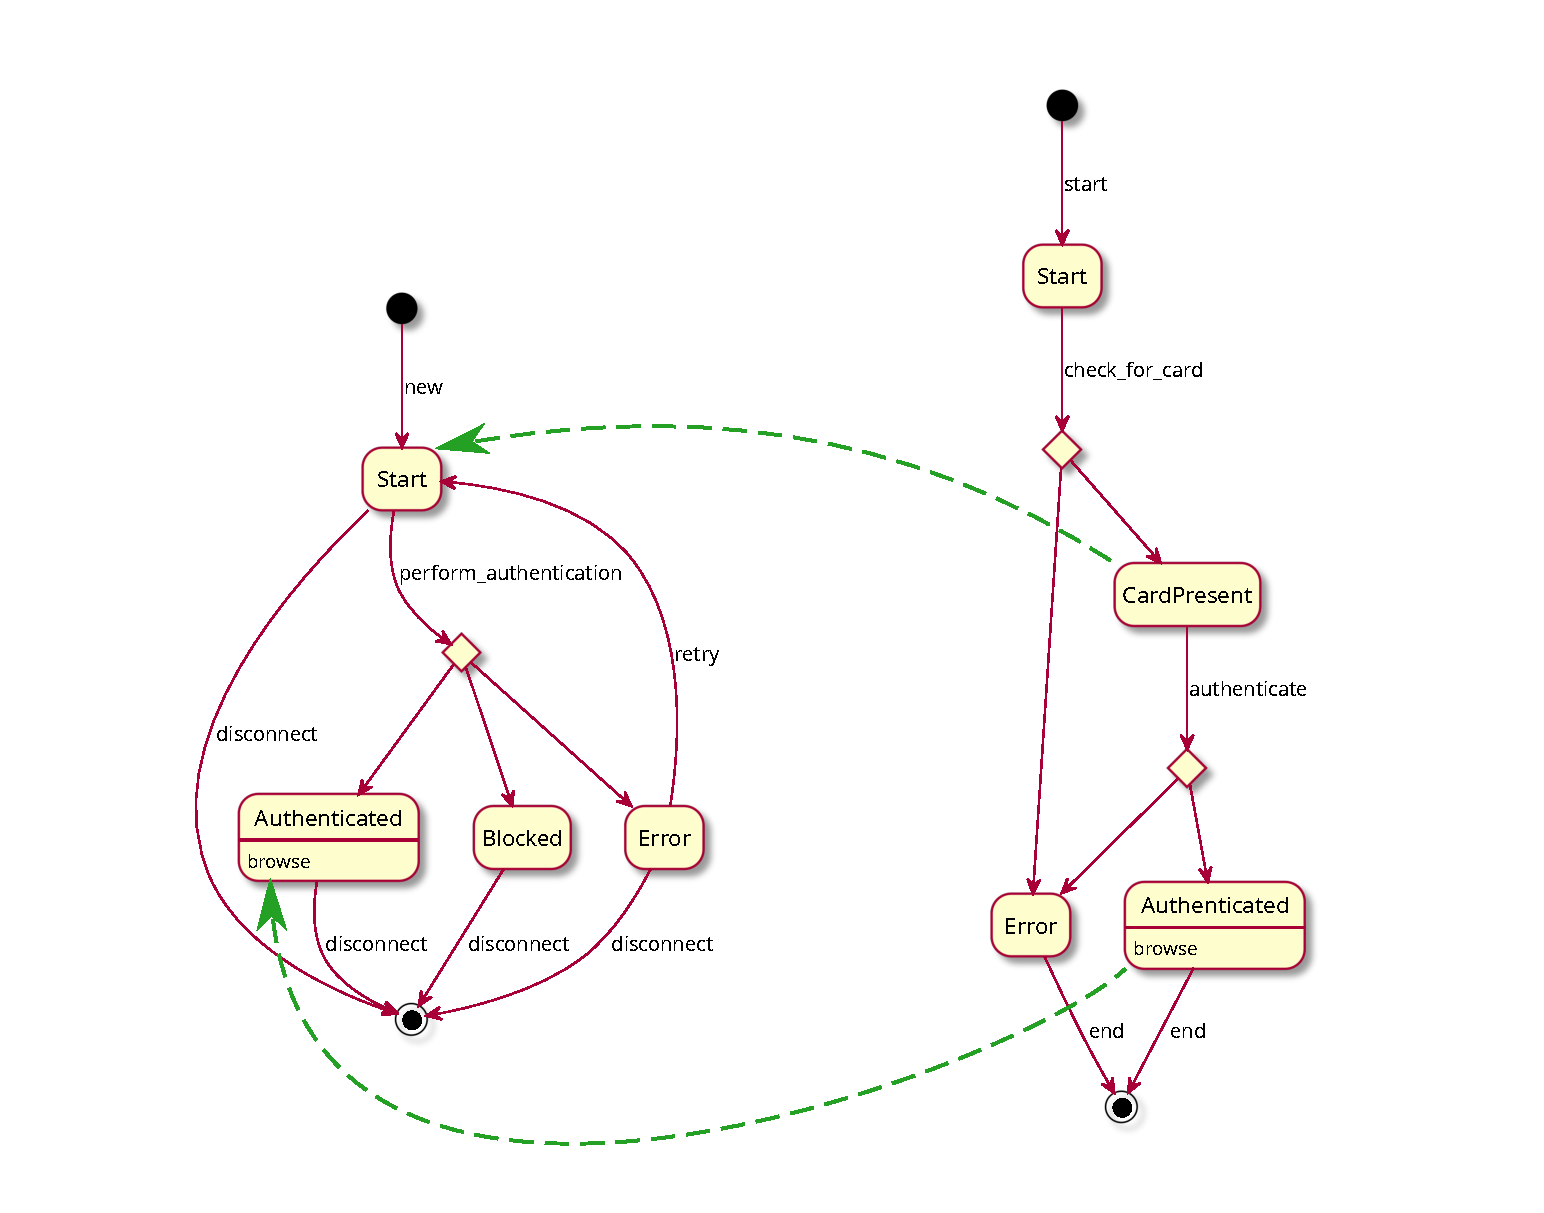
\includegraphics[width=\linewidth]{Chapters/Figures/C5/reader_typestates.pdf}
    \caption{
        The \textcolor{structblue}{\ttt{Reader}} and \textcolor{structblue}{\ttt{Card}} typestates,
        the green arrows indicate the dependency relationship between states.
    }
    \label{fig:reader-card-typestates}
\end{figure}

\begin{listing}
    \begin{minted}{rust}
#[typestate]
pub mod reader_api {
    use crate::card::card_api;

    #[automaton] pub struct Reader;

    #[state] pub struct Start;
    pub trait Start {
        fn start() -> Start;
        fn check_for_card(self) -> CheckCardResult;
    }

    #[state] pub struct CardPresent {
        pub card: card_api::Card<card_api::Start>,
    }
    pub trait CardPresent {
        fn authenticate(self, pin: [u8; 4]) -> AuthResult;
    }

    #[state] pub struct Authenticated {
        pub card: card_api::Card<card_api::Authenticated>,
    }
    pub trait Authenticated {
        fn browse(&self);
        fn end(self);
    }

    #[state] pub struct Error {
        pub message: String,
    }
    pub trait Error {
        fn end(self);
    }

    pub enum CheckCardResult { CardPresent, Error }
    pub enum AuthResult { Authenticated, Error }
}
    \end{minted}
    \caption{The \textcolor{structblue}{\texttt{Reader}} typestate specification.}
    \label{lst:typestate-reader}
\end{listing}

\begin{listing}
    \begin{minted}{rust}
#[typestate]
pub mod card_api {
    #[automaton] pub struct Card {
        pub valid_pin: [u8; 4],
        pub attempts_left: u8,
    }

    #[state] pub struct Start;
    pub trait Start {
        fn new() -> Start;
        fn perform_authentication(self, pin: [u8; 4]) -> AuthResult;
        fn disconnect(self);
    }

    #[state] pub struct Authenticated;
    pub trait Authenticated {
        fn browse(&self);
        fn disconnect(self);
    }

    #[state] pub struct Error;
    pub trait Error {
        fn retry(self) -> Start;
        fn disconnect(self);
    }

    #[state] pub struct Blocked;
    pub trait Blocked {
        fn disconnect(self);
    }

    pub enum AuthResult { Authenticated, Blocked, Error }
}
    \end{minted}
    \caption{The \textcolor{structblue}{\texttt{Card}} typestate specification.}
    \label{lst:typestate-card}
\end{listing}


\section{Auction Client}\label{sec:case-study:auction}

This example showcases how one can build a typestated API on top of an existing \emph{non-typestated} API,
enhancing the guarantees provided by latter.
Its goal is to ensure that the user does not perform non-optimal bids \ie{only bids higher than the existing one}
in the case the user is outbid by another, the client is then required to withdraw its bid before submitting another.

The auction API is listed in \autoref{lst:typestate-auction},
it allows bidding to be done and to emulate the closure of the auction with each bid a random boolean is generated,
if the auction closes, bidding is closed; all checks are performed at runtime.

The client is required to check if the auction is running before any action can be performed.
This is done through the \ttt{has\_ended} function (line 13 of \autoref{lst:typestate-auction-client}),
which returns the \textcolor{structblue}{\ttt{AuctionState}} state (line 46 of \autoref{lst:typestate-auction-client}),
an enumeration representing the two possible outcomes of the transition;
in case the auction has ended, the only thing the user can do is end its \quotes{session};
otherwise the user will be placed in the \textcolor{structblue}{\ttt{NoBids}} state, as they have not submitted any bids.
From the \textcolor{structblue}{\ttt{NoBids}} state, the user can perform a bid;
in the case that the bid is not the highest, the user is forced to withdraw its bid;
if the bid is the highest the user can then check if their bid is still the highest or if the auction has ended.
In the case that the user's bid is no longer the highest, the user transitions into the \textcolor{structblue}{\ttt{Withdraw}} state again;
in the case that the auction has ended, the user will then check if they have won the auction or not,
and take the according action before ending the \quotes{session}.


\begin{listing}
    \begin{minted}{rust}
pub struct Auction {
    owner: String,
    bids: HashMap<String, u64>,
    highest_bid: u64,
    ended: bool,
}

impl Auction {
    pub fn new(owner: String) -> Self {
        Self {
            owner,
            bids: HashMap::new(),
            highest_bid: 0,
            ended: false,
        }
    }

    pub fn bid(&mut self, client: String, bid: u64) -> Option<()> {
        if self.owner != client && !self.has_ended() {
            self.ended = rand::random(); // simulate uncertainty
            self.bids.insert(client, bid);
            if self.highest_bid < bid {
                self.highest_bid = bid;
            }
            Some(())
        } else {
            None
        }
    }

    pub fn is_highest_bid(&self, client: &String) -> bool {
        match self.bids.get(client).map(|bid| self.highest_bid == *bid) {
            Some(is_highest) => is_highest,
            None => false,
        }
    }

    pub fn get_bid(&self, client: String) -> Option<&u64> {
        self.bids.get(&client)
    }

    pub fn has_ended(&self) -> bool { self.ended }
}
    \end{minted}
    \caption{The auction \emph{non-typestated} API.}
    \label{lst:typestate-auction}
\end{listing}

\begin{listing}
    \begin{minted}{rust}
#[typestate]
mod auction_client_api {
    use crate::auction::Auction;

    #[automaton] pub struct Client {
        pub(crate) name: String,
        pub(crate) auction: Auction,
    }

    #[state] pub struct AuctionRunning;
    pub trait AuctionRunning {
        fn start(name: String, auction: Auction) -> AuctionRunning;
        fn has_ended(self) -> AuctionState;
    }

    #[state] pub struct NoBids;
    pub trait NoBids {
        fn bid(self, bid: u64) -> BidStatus;
    }

    #[state] pub struct HasBidded;
    pub trait HasBidded {
        fn check_bid(self) -> BidStatus;
        fn has_ended(self) -> AuctionEnded;
    }

    #[state] pub struct CheckWinner;
    pub trait CheckWinner { fn is_highest_bid(self) -> WinnerStatus; }

    #[state] pub struct Withdraw;
    pub trait Withdraw { fn withdraw(self) -> AuctionRunning; }

    #[state] pub struct Lost;
    pub trait Lost { fn withdraw(self) -> End; }

    #[state] pub struct Winner;
    pub trait Winner { fn win(self) -> End; }

    #[state] pub struct End;
    pub trait End { fn end(self); }

    pub enum WinnerStatus { Lost, Winner }

    pub enum AuctionEnded { HasBidded, CheckWinner }

    pub enum AuctionState { NoBids, End }

    pub enum BidStatus { HasBidded, Withdraw }
}
    \end{minted}
    \caption{The auction client's typestate declaration.}
    \label{lst:typestate-auction-client}
\end{listing}

\begin{figure}
    \centering
    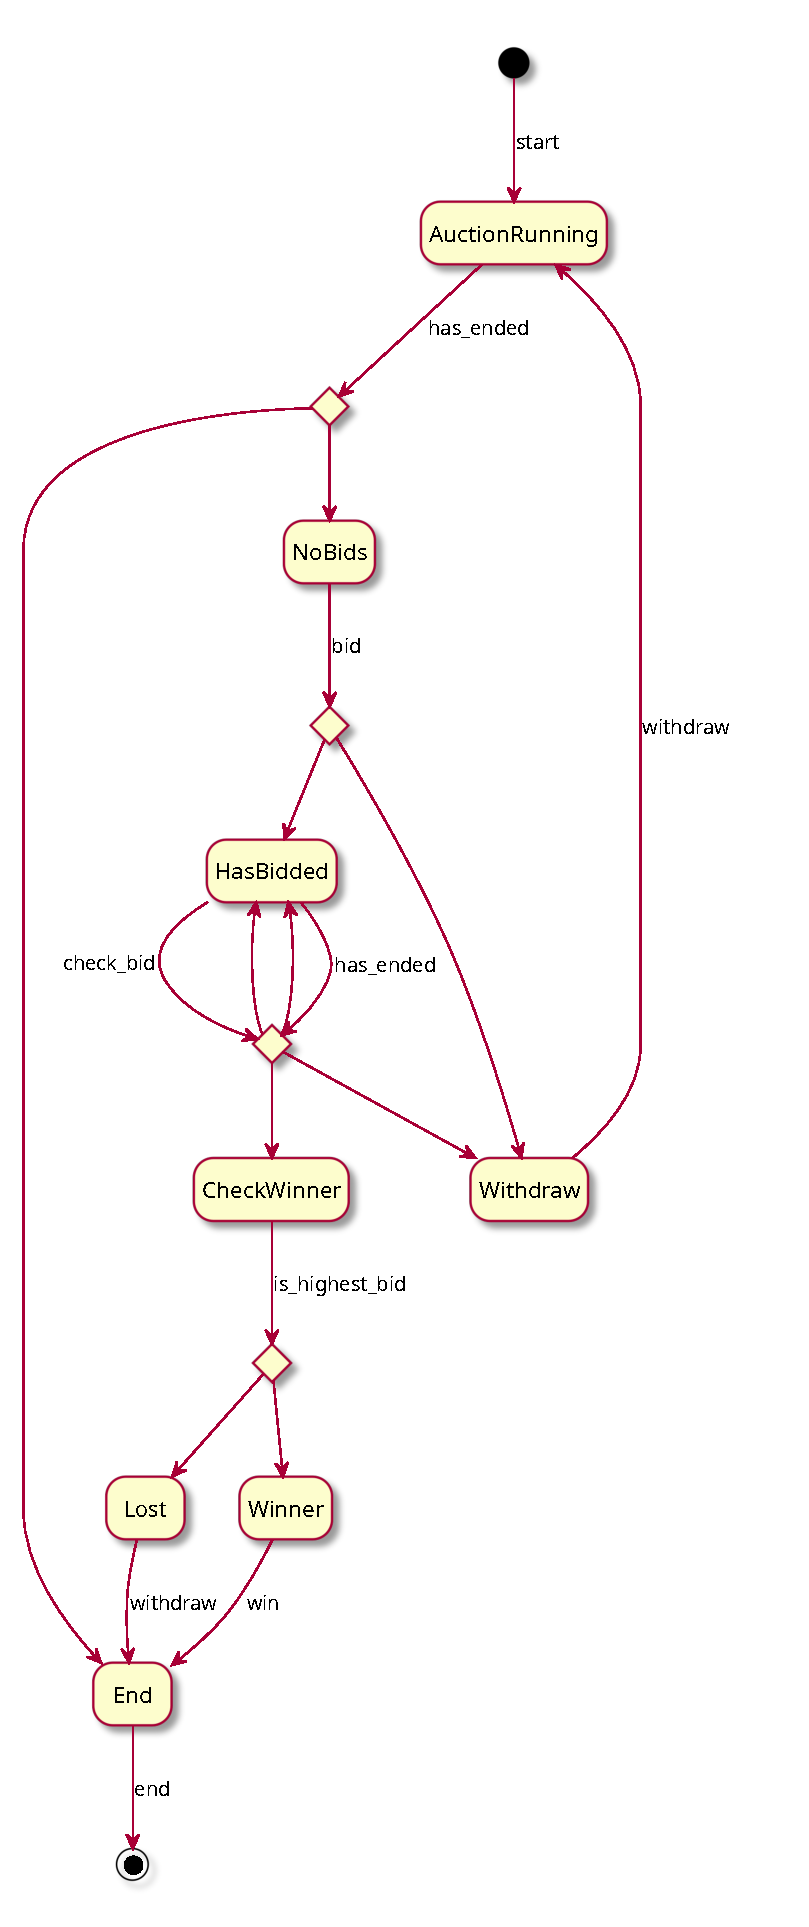
\includegraphics[width=0.6\linewidth]{Chapters/Figures/C5/auction_client.pdf}
    \caption{The auction client's typestate.}
    \label{fig:auction-typestate}
\end{figure}

\section{Summary}

In this chapter I have presented three examples which highlight different capabilities of the \textcolor{attrgreen}{\annotation{typestate}} macro.
The first example (\autoref{sec:case-study:ring}) shows how \textcolor{attrgreen}{\annotation{typestate}} is able to constrain the behavior of objects in multi threaded environments;
the second example (\autoref{sec:case-study:pin}) highlights how using multiple typestates in conjunction allows the developer to provide extra guarantees,
especially when compared with non-typestated APIs;
finally, the final example (\autoref{sec:case-study:auction}) illustrates how one can wrap an existing API using \textcolor{attrgreen}{\annotation{typestate}}
to provide a safe-to-use API.

While in some cases one can further abstract over the code written using \textcolor{attrgreen}{\annotation{typestate}},
such cases are often trivial to address using Rust's \ttt{macro\_rules!}.
Overall, \textcolor{attrgreen}{\annotation{typestate}} is able to address the problem at hand and
allow the developer to write an elegant solution while providing the desired API constraints.